% Pontos A(0,0), B(2,0), C(4,0), D(0,-1.5), E(2,-1.5), F(4,-1.5)
% Vigas AB, BC, CF, FE, ED, DA, BD, BE, BF
% Apoio móvel em D, apoio fixo em F
% 10kN aplicada para baixo em A, 6kN aplicada para direita em A
% 5kN aplicado para baixo em B, 10kN aplicado para baixo em C

\documentclass[tikz]{standalone}
\usepackage{stanli}
\usetikzlibrary{calc}

\begin{document}
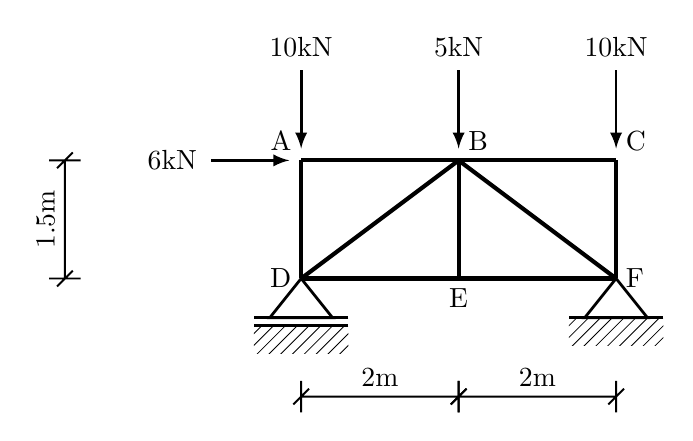
\begin{tikzpicture}
    % Definição dos pontos
    \point{A}{0}{0}
    \point{B}{2}{0}
    \point{C}{4}{0}
    \point{D}{0}{-1.5}
    \point{E}{2}{-1.5}
    \point{F}{4}{-1.5}

    % Definição das vigas/barras
    \beam{2}{A}{B}
    \beam{2}{B}{C}
    \beam{2}{C}{F}
    \beam{2}{F}{E}
    \beam{2}{E}{D}
    \beam{2}{D}{A}
    \beam{2}{B}{D}
    \beam{2}{B}{E}
    \beam{2}{B}{F}

    % Apoios
    \support{2}{D} % Apoio móvel em D
    \support{1}{F} % Apoio fixo em F

    % Cargas pontuais
    % A: 10kN para baixo (90) e 6kN para direita (180)
    \load{1}{A}[90]
    \load{1}{A}[180]
    
    % B: 5kN para baixo (90)
    \load{1}{B}[90]
    
    % C: 10kN para baixo (90)
    \load{1}{C}[90]

    % Notações de cargas e pontos
    \notation{1}{A}{A}[above left]
    \notation{1}{B}{B}[above right]
    \notation{1}{C}{C}[above right]
    \notation{1}{D}{D}[left]
    \notation{1}{E}{E}[below]
    \notation{1}{F}{F}[right]

    % Etiquetas de valores das cargas (conforme regras de offset)
    \notation{1}{A}{10kN}[above=12mm]
    \notation{1}{A}{6kN}[left=12mm]
    \notation{1}{B}{5kN}[above=12mm]
    \notation{1}{C}{10kN}[above=12mm]

    % Dimensionamento
    % Horizontal (distância negativa para ficar abaixo da estrutura)
    \dimensioning{1}{D}{E}{-30mm}[2m]
    \dimensioning{1}{E}{F}{-30mm}[2m]
    
    % Vertical (distância negativa para ficar à esquerda, compensando a carga em A)
    \dimensioning{2}{D}{A}{-30mm}[1.5m]

\end{tikzpicture}
\end{document}